\begin{abox}
	Practice Set-2\\ \vspace{0.2cm} Electric Potential
\end{abox}
\begin{enumerate}
\item An insulating sphere of radius $a$ carries a charge density
$$
\rho(\vec{r})=\rho_{0}\left(a^{2}-r^{2}\right) \cos \theta ; r<a
$$
The leading order term for the electric field at a distance $d$, far away from the charge distribution, is proportional to
{\exyear{GATE 2010}}

\begin{tasks}(4)
\task[\textbf{A.}] $d^{-1}$
\task[\textbf{B.}] $d^{-2}$
\task[\textbf{C.}] $d^{-3}$
\task[\textbf{D.}] $d^{-4}$
\end{tasks}	
\begin{answer}
	\begin{align*}
	V(r)&=\left[\frac{1}{r} \int_{V} \rho d \tau+\frac{1}{r^{2}} \int \rho \cos \theta d \tau+\cdots\right]\\
	\mathrm{I}^{\mathrm{st}}\text{ term, }\int \rho d \tau&=\int_{0}^{a} \int_{0}^{\pi} \int_{0}^{2 \pi} \rho_{0}\left(a^{2}-r^{2}\right) \cos \theta \times r^{2} \sin \theta d r d \theta d \phi=0\\
	\mathrm{II}^{\mathrm{nd}}\text{ term, }\int \rho \cos \theta d \tau&=\int_{0}^{a} \int_{0}^{\pi} \int_{0}^{2 \pi} \rho_{0}\left(a^{2}-r^{2}\right) \cos ^{2} \theta \times r^{2} \sin \theta d r d \theta d \phi \neq 0\\
	&\Rightarrow \mathrm{V} \alpha \frac{1}{\mathrm{r}^{2}} \Rightarrow E \alpha \frac{1}{\mathrm{r}^{3}}
	\end{align*}
	So the correct answer is \textbf{Option (C)}
\end{answer}
\item Two charges $q$ and $2 q$ are placed along the $x$ -axis in front of a grounded, infinite conducting plane, as shown in the figure. They are located respectively at a distance of $0.5 \mathrm{~m}$ and $1.5 \mathrm{~m}$ from the plane. The force acting on the charge $q$ is
{\exyear{GATE 2011}}

\begin{figure}[H]
\centering
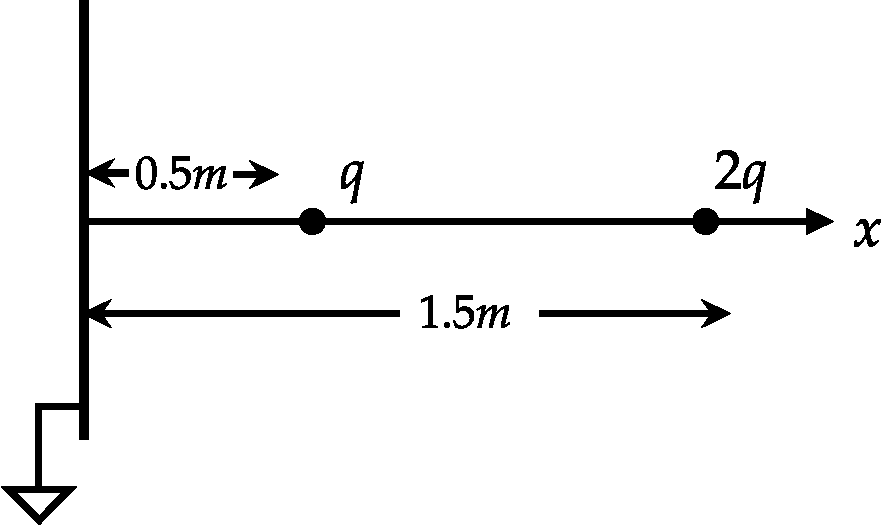
\includegraphics[height=4cm,width=7.5cm]{diagram-20210817(15)-crop}
\end{figure}
\begin{tasks}(4)
\task[\textbf{A.}] $\frac{1}{4 \pi \varepsilon_{0}} \frac{7 q^{2}}{2}$
\task[\textbf{B.}] $\frac{1}{4 \pi \varepsilon_{0}} 2 q^{2}$
\task[\textbf{C.}] $\frac{1}{4 \pi \varepsilon_{0}} q^{2}$
\task[\textbf{D.}] $\frac{1}{4 \pi \varepsilon_{0}} \frac{q^{2}}{2}$
\end{tasks}
\begin{answer}
	Using method of Images we can draw equivalent figure as shown below:\\
	\begin{figure}[H]
		\centering
		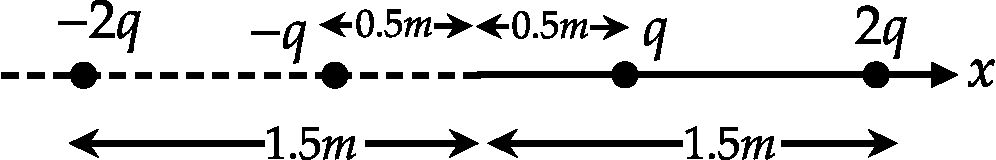
\includegraphics[height=1.2cm,width=9cm]{diagram-20210817(16)-crop}
	\end{figure}
	\begin{align*}
	F&=\frac{q}{4 \pi \varepsilon_{0}}\left[\frac{2 q}{(1)^{2}}+\frac{q}{(1)^{2}}+\frac{2 q}{(2)^{2}}\right]\\&=\frac{q}{4 \pi \varepsilon_{0}} \times \frac{7 q}{2}\\&=\frac{1}{4 \pi \varepsilon_{0}} \frac{7 q^{2}}{2}
	\end{align*}
	So the correct answer is \textbf{Option (A)}
\end{answer}
\item A spherical conductor of radius $a$ is placed in a uniform electric field $\vec{E}=E_{0} \hat{k}$. The potential at a point $P(r, \theta)$ for $r>a$, is given by
$$
\Phi(r, \theta)=\text { constant }-E_{0} r \cos \theta+\frac{E_{0} a^{3}}{r^{2}} \cos \theta
$$
where $r$ is the distance of $P$ from the centre $\mathrm{O}$ of the sphere and $\theta$ is the angle OP makes with the $z$ -axis The charge density on the sphere at $\theta=30^{\circ}$ is
{\exyear{GATE 2011}}

\begin{figure}[H]
\centering
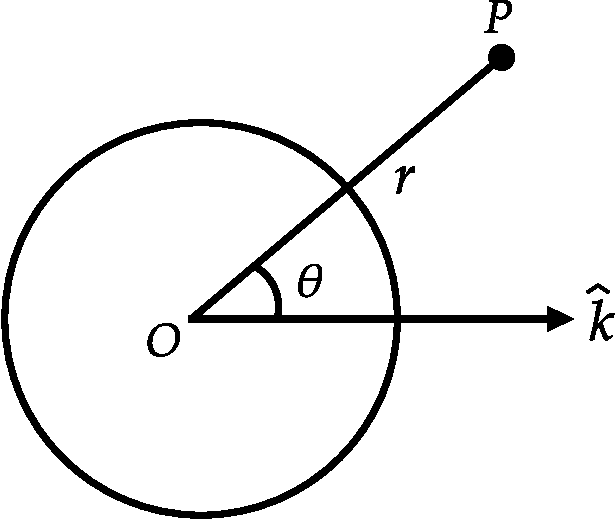
\includegraphics[height=4.2cm,width=5cm]{diagram-20210817(17)-crop}
\end{figure}
\begin{tasks}(4)
\task[\textbf{A.}] $3 \sqrt{3} \varepsilon_{0} E_{0} / 2$
\task[\textbf{B.}] $3 \varepsilon_{0} E_{0} / 2$
\task[\textbf{C.}] $\sqrt{3} \varepsilon_{0} E_{0} / 2$
\task[\textbf{D.}] $\varepsilon_{0} E_{0} / 2$
\end{tasks}
\begin{answer}
	\begin{align*}
	\sigma&=-\left.\varepsilon_{0} \frac{\partial V}{\partial r}\right|_{r=a}\\&=-\varepsilon_{0}\left[-E_{0} \cos \theta-\frac{2 E_{0} a^{3}}{r^{3}} \cos \theta\right]_{r=a}\\
	\sigma&=-\varepsilon_{0}\left[-E_{0} \cos \theta-2 E_{0} \cos \theta\right] \Rightarrow \sigma\\&=+3 E_{0} \varepsilon_{0} \cos \theta=+3 E_{0} \varepsilon_{0} \cos 30^{\circ}\\&=\frac{3 \sqrt{3}}{2} \varepsilon_{0} E_{0}
	\end{align*}
	So the correct answer is \textbf{Option (A)}
\end{answer}
	\item For a scalar function $\varphi$ satisfying the Laplace equation, $\vec{\nabla} \varphi$ has
{\exyear{GATE 2013}}

\begin{tasks}(2)
\task[\textbf{A.}] Zero curl and non-zero divergence
\task[\textbf{B.}] Non-zero curl and zero divergence
\task[\textbf{C.}] Zero curl and zero divergence
\task[\textbf{D.}]  Non-zero curl and non-zero divergence
\end{tasks}
\begin{answer}
	\begin{align*}
	\nabla^{2} \varphi&=0 \Rightarrow \vec{\nabla} \cdot(\vec{\nabla} \varphi)\\&=0\text{ and } \Rightarrow \vec{\nabla} \times(\vec{\nabla} \varphi)=0
	\end{align*}
	So the correct answer is \textbf{Option (C)}
\end{answer}
\item A charge distribution has the charge density given by $\rho=Q\left\{\delta\left(x-x_{0}\right)-\delta\left(x+x_{0}\right)\right\}$. For
this charge distribution the electric field at $\left(2 x_{0}, 0,0\right)$
{\exyear{GATE 2013}}

\begin{tasks}(4)
\task[\textbf{A.}] $\frac{2 Q \hat{x}}{9 \pi \varepsilon_{0} x_{0}^{2}}$
\task[\textbf{B.}] $\frac{Q \hat{x}}{4 \pi \varepsilon_{0} x_{0}^{3}}$
\task[\textbf{C.}] $\frac{Q \hat{x}}{4 \pi \varepsilon_{0} x_{0}^{2}}$
\task[\textbf{D.}] $\frac{Q \hat{x}}{16 \pi \varepsilon_{0} x_{0}^{2}}$
\end{tasks}
\begin{answer}
\begin{align*}
\text{	Potential }V(r)&=\frac{1}{4 \pi \varepsilon_{0}}\left[\int_{-a}^{a} \frac{\rho\left(x^{\prime}\right)}{x} d x^{\prime}+\int_{-a}^{a} \frac{\rho\left(x^{\prime}\right)}{x^{2}} x^{\prime} d x^{\prime}+\int_{-a}^{a} \frac{\rho\left(x^{\prime}\right)}{x^{3}} x^{\prime 2} d x^{\prime}+\ldots .\right]
\intertext{First term, total charge}
Q_{T}&=\int \rho\left(x^{\prime}\right) d x^{\prime}=Q \int_{-x_{0}}^{x_{0}} \delta\left(x^{\prime}-x_{0}\right) d x^{\prime}-Q \int_{-x_{0}}^{x_{0}} \delta\left(x^{\prime}+x_{0}\right) d x^{\prime}\\&=Q-Q=0
\intertext{Second term, dipole moment}
p&=\int x^{\prime} \rho\left(x^{\prime}\right) d x^{\prime}=Q \int_{-x_{0}}^{x_{0}} x^{\prime} \delta\left(x^{\prime}-x_{0}\right) d x^{\prime}-Q \int_{-x_{0}}^{x_{0}} x^{\prime} \delta\left(x^{\prime}+x_{0}\right) d x^{\prime}\\&=Q x_{0}-Q \times-x_{0}=2 Q x_{0}\\
V&=\frac{2 Q x_{0}}{4 \pi \varepsilon_{0} x^{2}} \Rightarrow \vec{E}=-\frac{\partial V}{\partial x} \hat{x}\\&=\frac{4 Q x_{0}}{4 \pi \varepsilon_{0} x^{3}} \hat{x}=\frac{4 Q x_{0}}{4 \pi \varepsilon_{0}\left(2 x_{0}\right)^{3}} \hat{x}\\&=\frac{Q}{8 \pi \varepsilon_{0} x_{0}^{2}} \hat{x}
\end{align*}
\end{answer}
	\item A charge $-q$ is distributed uniformly over a sphere, with a positive charge $q$ at its center in (i). Also in (ii), a charge $-q$ is distributed uniformly over an ellipsoid with a positive charge $q$ at its center. With respect to the origin of the coordinate system, which one of the following statements is correct?
{\exyear{GATE 2015}}

\begin{figure}[H]
\centering
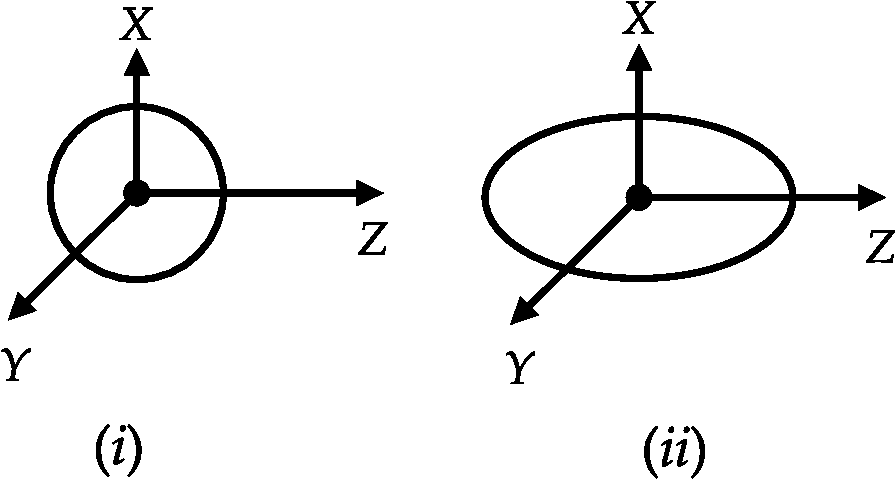
\includegraphics[height=5cm,width=10cm]{diagram-20210818(7)-crop}
\end{figure}
\begin{tasks}(1)
\task[\textbf{A.}] The dipole moment is zero in both (i) and (ii)
\task[\textbf{B.}] The dipole moment is non-zero in (i) but zero in (ii)
\task[\textbf{C.}] The dipole moment is zero in (i) but non-zero in (ii)
\task[\textbf{D.}] The dipole moment is non-zero in both (i) and (ii)
\end{tasks}
\begin{answer}
\begin{align*}
\vec{p}=\sum q_{i} \vec{r}_{i}=0\text{ in both cases.}
\end{align*}
So the correct answer is \textbf{Option (A)}
\end{answer}
	\item Identical charges $q$ are placed at five vertices of a regular hexagon of side $a$. The magnitude of the electric field and the electrostatic potential at the centre of the hexagon are respectively
{\exyear{GATE 2017}}

\begin{tasks}(4)
\task[\textbf{A.}] 0,0
\task[\textbf{B.}] $\frac{q}{4 \pi \varepsilon_{0} a^{2}}, \frac{q}{4 \pi \varepsilon_{0} a}$
\task[\textbf{C.}] $\frac{q}{4 \pi \varepsilon_{0} a^{2}}, \frac{5 q}{4 \pi \varepsilon_{0} a}$
\task[\textbf{D.}]  $\frac{\sqrt{5} q}{4 \pi \varepsilon_{0} a^{2}}, \frac{\sqrt{5} q}{4 \pi \varepsilon_{0} a}$
\end{tasks}
\begin{answer}
\begin{figure}[H]
	\centering
	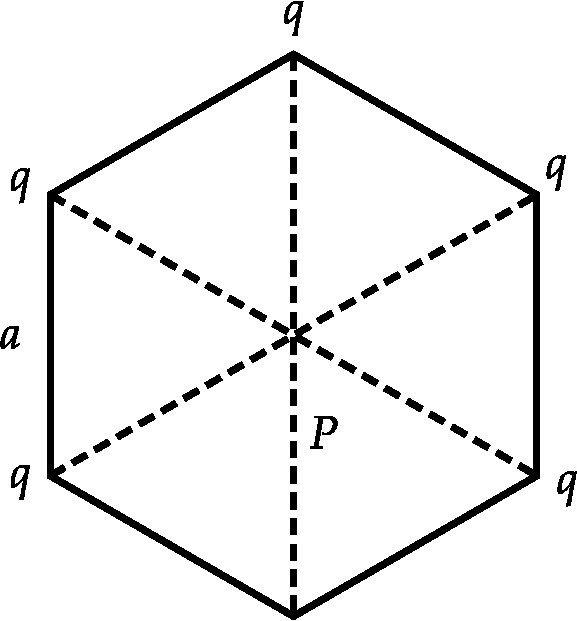
\includegraphics[height=4.3cm,width=4cm]{diagram-20210818(10)-crop}
\end{figure}
\begin{align*}
\text{The resultant field at }\mathrm{P}\text{ is }E&=\frac{q}{4 \pi \varepsilon_{0} a^{2}}\\
\text{The electrostatic potential at }\mathrm{P}\text{ is }V&=\frac{5 q}{4 \pi \varepsilon_{0} a}
\end{align*}
So the correct answer is \textbf{Option (C)}
\end{answer}
	\item Three charges $(2 C,-1 C,-1 C)$ are placed at the vertices of an equilateral triangle of side $1 m$ as shown in the figure. The component of the electric dipole moment about the marked origin along the $\hat{y}$ direction is-------$C m$.
{\exyear{GATE 2017}}

\begin{figure}[H]
\centering
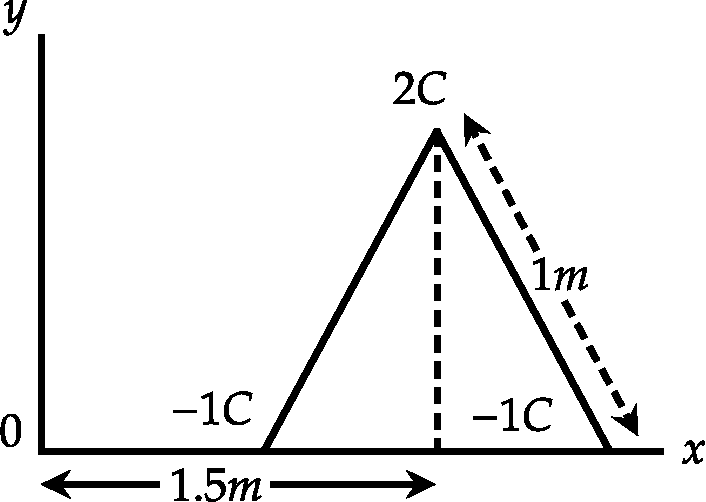
\includegraphics[height=4.5cm,width=6cm]{diagram-20210818(11)-crop}
\end{figure}
\begin{answer}
\begin{align*}
\vec{p}&=-1(1 \hat{x})-1(2 \hat{x})+2(1.5 \hat{x}+\sqrt{1-0.25} \hat{y})\\
\text{	Along the }\hat{y}\text{ direction }&=2 \times \sqrt{1-0.25}=1.73
\end{align*}
\end{answer}
\end{enumerate}
